\chapter{Design and Implementation}\label{ch:design}

\section{Multiplexer Policy}

We design several different multiplexers, each implementing a different policy
that only seeks to cater to specific use cases. The multiplexers are trusted components,
and thus are kept intentionally simple to leave them accessible to formal verification.
The main tasks of the multiplexers, regardless of policy implemented, are as follows:

\begin{itemize}
    \item Given a virtual address from the client/copier, translate it to a phyiscal address before
            handing it over to the driver.
    \item Given a physical address from the driver, translate it to a virtual address before
            handing it over to the client/copier.
    \item Sanitise any buffer addresses from the client before forwarding them.
    \item Sanitise any addresses from the driver. 
    \item Transmit buffers belong to the client, and all free buffers on the transmit path
            must be returned to the appropriate client.
    \item Receive buffers belong to the driver, and all free buffers on the receive path
            must be returned to the driver.
    \item Implement policy as detailed below.
    \item The transmit multiplexer must sanitise the ethernet header of outgoing packets
          to ensure the destination MAC address is well formed and will not cause issues
          on the network. 
\end{itemize}


\subsection{Receive Policy}

All incoming packets are processed in FIFO order. The multiplexer contains a 
mapping of virtualised client MAC addresses and client queues. After dequeuing an incoming packet,
the multiplexer must first invalidate the cache (to ensure subsequent reads are fetched again from memory)
and read the packet header. The packet header contains the destination MAC address and if the packet is
addressed to a client on the system, the buffer address is forwarded to the appropriate client. 
If a clients receive used queue is full, the packet is dropped and the buffer address is returned to
the driver. This can be prevented for higher priority clients by appropriate choice of clients receive
used queue sizes. Appropriate sizes can be selected based on experients discussed in \autoref{ch:evaluation}.

The multiplexer must also return free buffers to the driver to be reused again. If a clients receive free
queue is full, it could stall the client while it waits to enqueue free buffers. Should this be the case,
the order in which the multiplexer processes the client receive free queues contains policy as it may
unblock clients. We propose instead to ensure the clients receive free queue is the same size as the number
of receive buffers circulating and thus prevent the client becoming blocked on waiting for this queue to be
processed. This design removes the need for policy on processing free buffers. \\ 

\subsection{Transmit Policy}

All incoming requests from clients are processed given a particular policy. The designs of each policy
are outlined below.\\
The transmit multiplexer returns free buffers from the driver to the client in FIFO order.
We propose client transmit free queues are at least the size of the number of buffers
belonging to that client in order to prevent the multiplexer from becoming blocked 
should a clients free queue become full. \\ 
Similarly, the drivers transmit used queue should be at least the size of the sum of 
all client transmit buffers. This ensures the multiplexer will not become blocked on this queue
and thus disrupt the policy implemented to process client requests. \\ 

\subsubsection{Round Robin Policy}
We implement a round robin policy by processing a single clients transmit request at a time.
This is done in a loop to ensure we process any batched requests as outlined in \autoref{l:roundrobin}.

\begin{lstlisting}[tabsize=2, language=C, caption={Transmit Round Robin Policy},frame=tb, 
                    label={l:roundrobin}, captionpos=b]
void process_transmit_ready():
    enqueued = 0
    old_enqueued = 0

    while(!ring_full(driver.used_ring)):
        old_enqueued = enqueued
        for each client:
            // Process a single used buffer at a time. 
            if (!ring_empty(client.used_ring) &&
                !ring_full(driver.used_ring)):
                buf = dequeue(client.used_ring)
                phys = get_phys_addr(buf)
                enqueue(driver.used_ring, phys)

                enqueued += 1
            
        /* we haven't processed any packets since 
            last loop, exit */
        if (old_enqueued == enqueued) break;
\end{lstlisting}

\subsubsection{Priority-based Policy}

We implement a priority based policy in \autoref{l:prioritybased}. We assume the list of
clients is ordered from highest priority to lowest. Thus it is possible to change a clients
priority at run time by manipulating this list.\\

\begin{minipage}{\textwidth}
    \centering
    \begin{lstlisting}[tabsize=2, language=C, caption={Transmit Priority-based Policy},frame=tb, 
                        label={l:prioritybased}, captionpos=b]
void process_transmit_ready():
    enqueued = 0
    old_enqueued = 0
    while(!ring_full(driver->used_ring)):
        old_enqueued = enqueued
        for client in clients:
            while(!ring_empty(client->used_ring) &&
                    !ring_full(driver->used_ring)):
                buf = dequeue(client.used_ring)
                phys = get_phys_addr(buf)
                enqueue(driver.used_ring, phys)

                enqueued += 1
                /* if a higher priority client has since 
                    made a request, go again */
                if (!ring_empty(clients[:client])): break

        if old_enqueued == new_enqueued: break
\end{lstlisting}
\end{minipage}

\subsubsection{Bandwidth Limited Policy}

We implement a bandwidth limited policy in \autoref{l:bandwidth}. This multiplexer must
also communicate with a timer driver to get the time and set timeouts. The timer driver
API is shown in \autoref{l:timer}.

\begin{minipage}{\textwidth}
    \centering
    \begin{lstlisting}[tabsize=2, language=C, caption={Transmit Bandwidth Limited Policy},frame=tb, 
                        label={l:bandwidth}, captionpos=b]
void process_transmit_ready():
    curr_time = get_time()
    for each client:
        if (curr_time - client.last_time >= TIME_WINDOW):
            client.last_time = curr_time
            client.bandwidth = 0
        
        while !ring_empty(client.used_ring) && 
                !ring_full(driver.used_ring) && 
                client.bandwidth < client.max:
            buf = dequeue(client.used_ring)
            phys = get_phys_addr(buf)
            enqueue(driver.used_ring, phys)
            /* recalculate the clients bandwidth used in 
                the current time period */ 
            client.bandwidth = calculate_bandwidth(buf_size)

        if !ring_empty(client.used_ring) && !client.timeout:
            request_timeout(TIME_WINDOW - curr_time - client.last_time)
            client.timeout = true
    \end{lstlisting}
\end{minipage}

\begin{minipage}{\textwidth}
    \centering
    \begin{lstlisting}[tabsize=2, language=C, caption={Timer Driver API},frame=tb, 
                        label={l:timer}, captionpos=b]
uint64_t get_time() {
    return sel4cp_ppcall(TIMER, sel4cp_msginfo_new(GET_TIME, 0));
}
        
void request_timeout(uint64_t micros) {
    sel4cp_mr_set(0, micros);
    sel4cp_ppcall(TIMER, sel4cp_msginfo_new(SET_TIMEOUT, 1));
}
    \end{lstlisting}
\end{minipage}

The timer driver is a high priority, passive server. It receives interrupts from the deveice,
and forwards these by notifying the appropriate client or multiplexer. Thus the bandwidth limited
multiplexer also reacts to such notifications by clearing the appropriate clients timeout and
recalling process\_transmit\_ready.

This bandwidth limited policy can also be combined with the round robin or priority based policy
to order each clients requests. Such a case would be useful in reducing/limited the 
transmit latencies of latency sensitive applications.\\ 

% does it make sense to set a total limit greater than whats actually available? 

\subsection{Enforcing Policy Through System Design}
Depending on the greater system design, we expect some transmit policies to not work.
For example, given a single core configuration, the higher priority multiplexer will
always be invoked as soon as a client has made a request to transmit. This means that
we can assume any other clients do not yet wish to transmit, or have not yet had the
opportunity to run to make a request. Therefore, the multiplexer does not need to 
consider all the client queues when invoked and can just service requests made
by the client which signalled. To enforce policy on multiple clients in such a scenario,
we rely on appropriate choices of client queue sizes and the scheduling parameters
of each client. For example, to enforce a round robin policy, we run both clients
at equal priorities, and limit their transmit used queues to just one. This ensures
that each client will be stalled until their single request has been processed, and
another client will have the opportunity to run in the interim. The multiplexer will
then only process a single request per client at a time.\\
Similarly, should we require a priority based policy, we can set appropriate priorities
to the clients scheduling contexts and rely on the scheduling of the system to reinforce
this policy.\\
Finally, we can limit the clients queue sizes on both the transmit and/or receive paths
to limit the amount of either transmit and/or receive throughput available to each client.
Appropriate sizes can be selected based on experients discussed in \autoref{ch:evaluation}.\\ 

\section{Broadcast Protocols}
Some protocols broadcast traffic to all systems by addressing the
ethernet packet with a specific MAC address of ff:ff:ff:ff. However,
as the receive multiplexer is based on MAC addresses, it will not
know how to handle such packets. In particular, we need to support 
the address resolution protocol (ARP), as it maps an
IPv4 address to a MAC address and thus 
is required for any network communication via ethernet.\\
One possible solution is to copy these packets to all client applications.
This would require additional policy in the receive multiplxer that ensures
all client side receive free (RxF) queues have enough free buffers available
for the multiplexer to dequeue and then copy broadcast packets into.
However, there are many different broadcast protocols, for example the Dynamic
Host Configuration Protocol (DHCP), and the arrival of such packets
can be nondeterministic. This makes it difficult to determine how many might arrive
simultaneously and thus how many buffers should be available in all client side
RxF queues at all times. If there aren't any free buffers available for ARP, then
a client will not be able to receive any IPv4 traffic.\\
Instead, we implement a separate component to handle broadcast traffic. It interfaces
with the multiplexers the same as any other client, as shown in \autoref{f:mux}. 

\begin{figure}[h]
    \centering
    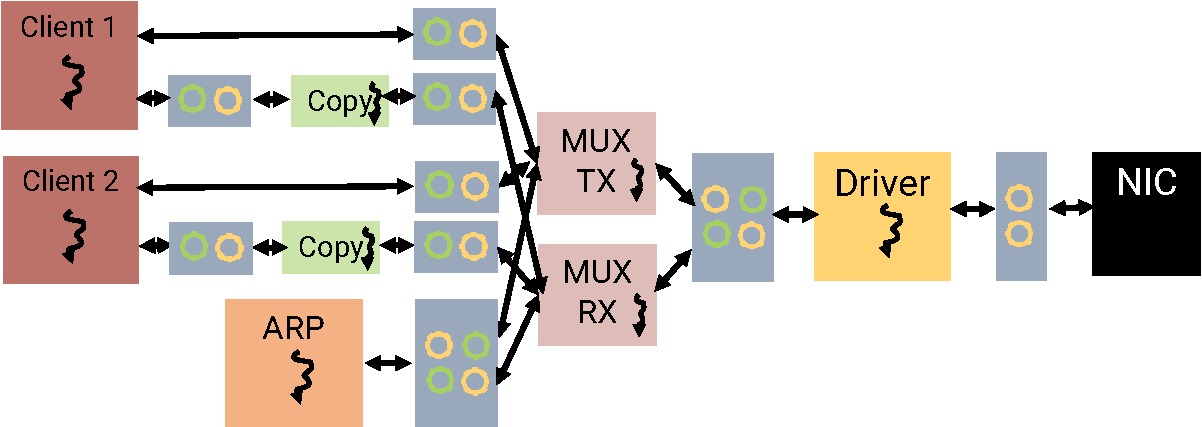
\includegraphics[width=\textwidth]{arp.pdf}
    \caption{Multiple client applications with an ARP component on the sDDF}
    \label{f:arp}
\end{figure}

\subsection{Separate ARP Component}
A separate ARP component only requries the minimal functionality to respond to 
the address resolution protocol on behalf of any client applications running on
the system. In keeping with the design goals, this component will be kept 
very simple in the aims of enabling formal verification. Therefore we consider
this component to be trusted to maintain the integrity of its shared queues with
the multiplexer components as well as interfacing with clients and responding
correctly to ARP on behalf of the clients. \\
While supporting other broadcast protocols, such as DHCP, is out of scope of this thesis, 
the simplicity of the ARP component design enables its functionality to be extended easily
to support other broadcast protocols in the future.

\subsection{Client Interface}
As ARP is based on both MAC addresses and IPv4 addresses, the new component
requires an interface with client applications. This interface will allow clients
to register a new IPv4 address, change an IPv4 address, or remove one. As adding,
changing and removing an IPv4 address is typically very infrequent for networking systems
and requires minimal data exchange, we define this interface using a protected procedure
call (PPC) from the client to the ARP component. 

\begin{minipage}{\textwidth}
    \fontsmall
    \centering
    \begin{lstlisting}[tabsize=2, language=C, caption={Client Interface to ARP Component},frame=tb, 
                        label={l:arpintf}, captionpos=b]
void register_ip4(new_ip4_addr, mac_addr[6])
{
    /* split the MAC address across two registers so it fits */
    sel4cp_mr_set(0, mac_addr[0:4]);
    sel4cp_mr_set(1, mac_addr[4:6]);
    sel4cp_mr_set(2, new_ip4_addr);
    sel4cp_ppcall(ARP, sel4cp_msginfo_new(REGISTER_IP, 3));
}

void change_ip4(old_ip4_addr, new_ip4_addr, mac_addr[6])
{
    sel4cp_mr_set(0, mac_addr[0:4]);
    sel4cp_mr_set(1, mac_addr[4:6]);
    sel4cp_mr_set(2, old_ip4_addr);
    sel4cp_mr_set(3, new_ip4_addr);
    sel4cp_ppcall(ARP, sel4cp_msginfo_new(CHANGE_IP, 4));
}

void remove_ip4(old_ip4_addr, mac_addr[6])
{
    sel4cp_mr_set(0, mac_addr[0:4]);
    sel4cp_mr_set(1, mac_addr[4:6]);
    sel4cp_mr_set(2, old_ip4_addr);
    sel4cp_ppcall(ARP, sel4cp_msginfo_new(REMOVE_IP, 3));
}
    \end{lstlisting}
\end{minipage}

Currently, the ARP component can only store a single IPv4 address per client, which
is enough for our testing purposes, however this limit can be extended easily in the code
base should the need arise.\\

\section{Client Applications}

\subsection{Asymmetric Traffic}
% describe new client applications and test apps. 

\subsection{Client Initiated Transmit}
% describe client transmit benchmark. 

\section{Multicore systems}

\subsection{Two-threaded driver}
